
% Default to the notebook output style

    


% Inherit from the specified cell style.




    
\documentclass[11pt]{article}

    
    
    \usepackage[T1]{fontenc}
    % Nicer default font (+ math font) than Computer Modern for most use cases
    \usepackage{mathpazo}

    % Basic figure setup, for now with no caption control since it's done
    % automatically by Pandoc (which extracts ![](path) syntax from Markdown).
    \usepackage{graphicx}
    % We will generate all images so they have a width \maxwidth. This means
    % that they will get their normal width if they fit onto the page, but
    % are scaled down if they would overflow the margins.
    \makeatletter
    \def\maxwidth{\ifdim\Gin@nat@width>\linewidth\linewidth
    \else\Gin@nat@width\fi}
    \makeatother
    \let\Oldincludegraphics\includegraphics
    % Set max figure width to be 80% of text width, for now hardcoded.
    \renewcommand{\includegraphics}[1]{\Oldincludegraphics[width=.8\maxwidth]{#1}}
    % Ensure that by default, figures have no caption (until we provide a
    % proper Figure object with a Caption API and a way to capture that
    % in the conversion process - todo).
    \usepackage{caption}
    \DeclareCaptionLabelFormat{nolabel}{}
    \captionsetup{labelformat=nolabel}

    \usepackage{adjustbox} % Used to constrain images to a maximum size 
    \usepackage{xcolor} % Allow colors to be defined
    \usepackage{enumerate} % Needed for markdown enumerations to work
    \usepackage{geometry} % Used to adjust the document margins
    \usepackage{amsmath} % Equations
    \usepackage{amssymb} % Equations
    \usepackage{textcomp} % defines textquotesingle
    % Hack from http://tex.stackexchange.com/a/47451/13684:
    \AtBeginDocument{%
        \def\PYZsq{\textquotesingle}% Upright quotes in Pygmentized code
    }
    \usepackage{upquote} % Upright quotes for verbatim code
    \usepackage{eurosym} % defines \euro
    \usepackage[mathletters]{ucs} % Extended unicode (utf-8) support
    \usepackage[utf8x]{inputenc} % Allow utf-8 characters in the tex document
    \usepackage{fancyvrb} % verbatim replacement that allows latex
    \usepackage{grffile} % extends the file name processing of package graphics 
                         % to support a larger range 
    % The hyperref package gives us a pdf with properly built
    % internal navigation ('pdf bookmarks' for the table of contents,
    % internal cross-reference links, web links for URLs, etc.)
    \usepackage{hyperref}
    \usepackage{longtable} % longtable support required by pandoc >1.10
    \usepackage{booktabs}  % table support for pandoc > 1.12.2
    \usepackage[inline]{enumitem} % IRkernel/repr support (it uses the enumerate* environment)
    \usepackage[normalem]{ulem} % ulem is needed to support strikethroughs (\sout)
                                % normalem makes italics be italics, not underlines
    

    
    
    % Colors for the hyperref package
    \definecolor{urlcolor}{rgb}{0,.145,.698}
    \definecolor{linkcolor}{rgb}{.71,0.21,0.01}
    \definecolor{citecolor}{rgb}{.12,.54,.11}

    % ANSI colors
    \definecolor{ansi-black}{HTML}{3E424D}
    \definecolor{ansi-black-intense}{HTML}{282C36}
    \definecolor{ansi-red}{HTML}{E75C58}
    \definecolor{ansi-red-intense}{HTML}{B22B31}
    \definecolor{ansi-green}{HTML}{00A250}
    \definecolor{ansi-green-intense}{HTML}{007427}
    \definecolor{ansi-yellow}{HTML}{DDB62B}
    \definecolor{ansi-yellow-intense}{HTML}{B27D12}
    \definecolor{ansi-blue}{HTML}{208FFB}
    \definecolor{ansi-blue-intense}{HTML}{0065CA}
    \definecolor{ansi-magenta}{HTML}{D160C4}
    \definecolor{ansi-magenta-intense}{HTML}{A03196}
    \definecolor{ansi-cyan}{HTML}{60C6C8}
    \definecolor{ansi-cyan-intense}{HTML}{258F8F}
    \definecolor{ansi-white}{HTML}{C5C1B4}
    \definecolor{ansi-white-intense}{HTML}{A1A6B2}

    % commands and environments needed by pandoc snippets
    % extracted from the output of `pandoc -s`
    \providecommand{\tightlist}{%
      \setlength{\itemsep}{0pt}\setlength{\parskip}{0pt}}
    \DefineVerbatimEnvironment{Highlighting}{Verbatim}{commandchars=\\\{\}}
    % Add ',fontsize=\small' for more characters per line
    \newenvironment{Shaded}{}{}
    \newcommand{\KeywordTok}[1]{\textcolor[rgb]{0.00,0.44,0.13}{\textbf{{#1}}}}
    \newcommand{\DataTypeTok}[1]{\textcolor[rgb]{0.56,0.13,0.00}{{#1}}}
    \newcommand{\DecValTok}[1]{\textcolor[rgb]{0.25,0.63,0.44}{{#1}}}
    \newcommand{\BaseNTok}[1]{\textcolor[rgb]{0.25,0.63,0.44}{{#1}}}
    \newcommand{\FloatTok}[1]{\textcolor[rgb]{0.25,0.63,0.44}{{#1}}}
    \newcommand{\CharTok}[1]{\textcolor[rgb]{0.25,0.44,0.63}{{#1}}}
    \newcommand{\StringTok}[1]{\textcolor[rgb]{0.25,0.44,0.63}{{#1}}}
    \newcommand{\CommentTok}[1]{\textcolor[rgb]{0.38,0.63,0.69}{\textit{{#1}}}}
    \newcommand{\OtherTok}[1]{\textcolor[rgb]{0.00,0.44,0.13}{{#1}}}
    \newcommand{\AlertTok}[1]{\textcolor[rgb]{1.00,0.00,0.00}{\textbf{{#1}}}}
    \newcommand{\FunctionTok}[1]{\textcolor[rgb]{0.02,0.16,0.49}{{#1}}}
    \newcommand{\RegionMarkerTok}[1]{{#1}}
    \newcommand{\ErrorTok}[1]{\textcolor[rgb]{1.00,0.00,0.00}{\textbf{{#1}}}}
    \newcommand{\NormalTok}[1]{{#1}}
    
    % Additional commands for more recent versions of Pandoc
    \newcommand{\ConstantTok}[1]{\textcolor[rgb]{0.53,0.00,0.00}{{#1}}}
    \newcommand{\SpecialCharTok}[1]{\textcolor[rgb]{0.25,0.44,0.63}{{#1}}}
    \newcommand{\VerbatimStringTok}[1]{\textcolor[rgb]{0.25,0.44,0.63}{{#1}}}
    \newcommand{\SpecialStringTok}[1]{\textcolor[rgb]{0.73,0.40,0.53}{{#1}}}
    \newcommand{\ImportTok}[1]{{#1}}
    \newcommand{\DocumentationTok}[1]{\textcolor[rgb]{0.73,0.13,0.13}{\textit{{#1}}}}
    \newcommand{\AnnotationTok}[1]{\textcolor[rgb]{0.38,0.63,0.69}{\textbf{\textit{{#1}}}}}
    \newcommand{\CommentVarTok}[1]{\textcolor[rgb]{0.38,0.63,0.69}{\textbf{\textit{{#1}}}}}
    \newcommand{\VariableTok}[1]{\textcolor[rgb]{0.10,0.09,0.49}{{#1}}}
    \newcommand{\ControlFlowTok}[1]{\textcolor[rgb]{0.00,0.44,0.13}{\textbf{{#1}}}}
    \newcommand{\OperatorTok}[1]{\textcolor[rgb]{0.40,0.40,0.40}{{#1}}}
    \newcommand{\BuiltInTok}[1]{{#1}}
    \newcommand{\ExtensionTok}[1]{{#1}}
    \newcommand{\PreprocessorTok}[1]{\textcolor[rgb]{0.74,0.48,0.00}{{#1}}}
    \newcommand{\AttributeTok}[1]{\textcolor[rgb]{0.49,0.56,0.16}{{#1}}}
    \newcommand{\InformationTok}[1]{\textcolor[rgb]{0.38,0.63,0.69}{\textbf{\textit{{#1}}}}}
    \newcommand{\WarningTok}[1]{\textcolor[rgb]{0.38,0.63,0.69}{\textbf{\textit{{#1}}}}}
    
    
    % Define a nice break command that doesn't care if a line doesn't already
    % exist.
    \def\br{\hspace*{\fill} \\* }
    % Math Jax compatability definitions
    \def\gt{>}
    \def\lt{<}
    % Document parameters
    \title{Trematinib\_CI\_analysis}
    
    
    

    % Pygments definitions
    
\makeatletter
\def\PY@reset{\let\PY@it=\relax \let\PY@bf=\relax%
    \let\PY@ul=\relax \let\PY@tc=\relax%
    \let\PY@bc=\relax \let\PY@ff=\relax}
\def\PY@tok#1{\csname PY@tok@#1\endcsname}
\def\PY@toks#1+{\ifx\relax#1\empty\else%
    \PY@tok{#1}\expandafter\PY@toks\fi}
\def\PY@do#1{\PY@bc{\PY@tc{\PY@ul{%
    \PY@it{\PY@bf{\PY@ff{#1}}}}}}}
\def\PY#1#2{\PY@reset\PY@toks#1+\relax+\PY@do{#2}}

\expandafter\def\csname PY@tok@w\endcsname{\def\PY@tc##1{\textcolor[rgb]{0.73,0.73,0.73}{##1}}}
\expandafter\def\csname PY@tok@c\endcsname{\let\PY@it=\textit\def\PY@tc##1{\textcolor[rgb]{0.25,0.50,0.50}{##1}}}
\expandafter\def\csname PY@tok@cp\endcsname{\def\PY@tc##1{\textcolor[rgb]{0.74,0.48,0.00}{##1}}}
\expandafter\def\csname PY@tok@k\endcsname{\let\PY@bf=\textbf\def\PY@tc##1{\textcolor[rgb]{0.00,0.50,0.00}{##1}}}
\expandafter\def\csname PY@tok@kp\endcsname{\def\PY@tc##1{\textcolor[rgb]{0.00,0.50,0.00}{##1}}}
\expandafter\def\csname PY@tok@kt\endcsname{\def\PY@tc##1{\textcolor[rgb]{0.69,0.00,0.25}{##1}}}
\expandafter\def\csname PY@tok@o\endcsname{\def\PY@tc##1{\textcolor[rgb]{0.40,0.40,0.40}{##1}}}
\expandafter\def\csname PY@tok@ow\endcsname{\let\PY@bf=\textbf\def\PY@tc##1{\textcolor[rgb]{0.67,0.13,1.00}{##1}}}
\expandafter\def\csname PY@tok@nb\endcsname{\def\PY@tc##1{\textcolor[rgb]{0.00,0.50,0.00}{##1}}}
\expandafter\def\csname PY@tok@nf\endcsname{\def\PY@tc##1{\textcolor[rgb]{0.00,0.00,1.00}{##1}}}
\expandafter\def\csname PY@tok@nc\endcsname{\let\PY@bf=\textbf\def\PY@tc##1{\textcolor[rgb]{0.00,0.00,1.00}{##1}}}
\expandafter\def\csname PY@tok@nn\endcsname{\let\PY@bf=\textbf\def\PY@tc##1{\textcolor[rgb]{0.00,0.00,1.00}{##1}}}
\expandafter\def\csname PY@tok@ne\endcsname{\let\PY@bf=\textbf\def\PY@tc##1{\textcolor[rgb]{0.82,0.25,0.23}{##1}}}
\expandafter\def\csname PY@tok@nv\endcsname{\def\PY@tc##1{\textcolor[rgb]{0.10,0.09,0.49}{##1}}}
\expandafter\def\csname PY@tok@no\endcsname{\def\PY@tc##1{\textcolor[rgb]{0.53,0.00,0.00}{##1}}}
\expandafter\def\csname PY@tok@nl\endcsname{\def\PY@tc##1{\textcolor[rgb]{0.63,0.63,0.00}{##1}}}
\expandafter\def\csname PY@tok@ni\endcsname{\let\PY@bf=\textbf\def\PY@tc##1{\textcolor[rgb]{0.60,0.60,0.60}{##1}}}
\expandafter\def\csname PY@tok@na\endcsname{\def\PY@tc##1{\textcolor[rgb]{0.49,0.56,0.16}{##1}}}
\expandafter\def\csname PY@tok@nt\endcsname{\let\PY@bf=\textbf\def\PY@tc##1{\textcolor[rgb]{0.00,0.50,0.00}{##1}}}
\expandafter\def\csname PY@tok@nd\endcsname{\def\PY@tc##1{\textcolor[rgb]{0.67,0.13,1.00}{##1}}}
\expandafter\def\csname PY@tok@s\endcsname{\def\PY@tc##1{\textcolor[rgb]{0.73,0.13,0.13}{##1}}}
\expandafter\def\csname PY@tok@sd\endcsname{\let\PY@it=\textit\def\PY@tc##1{\textcolor[rgb]{0.73,0.13,0.13}{##1}}}
\expandafter\def\csname PY@tok@si\endcsname{\let\PY@bf=\textbf\def\PY@tc##1{\textcolor[rgb]{0.73,0.40,0.53}{##1}}}
\expandafter\def\csname PY@tok@se\endcsname{\let\PY@bf=\textbf\def\PY@tc##1{\textcolor[rgb]{0.73,0.40,0.13}{##1}}}
\expandafter\def\csname PY@tok@sr\endcsname{\def\PY@tc##1{\textcolor[rgb]{0.73,0.40,0.53}{##1}}}
\expandafter\def\csname PY@tok@ss\endcsname{\def\PY@tc##1{\textcolor[rgb]{0.10,0.09,0.49}{##1}}}
\expandafter\def\csname PY@tok@sx\endcsname{\def\PY@tc##1{\textcolor[rgb]{0.00,0.50,0.00}{##1}}}
\expandafter\def\csname PY@tok@m\endcsname{\def\PY@tc##1{\textcolor[rgb]{0.40,0.40,0.40}{##1}}}
\expandafter\def\csname PY@tok@gh\endcsname{\let\PY@bf=\textbf\def\PY@tc##1{\textcolor[rgb]{0.00,0.00,0.50}{##1}}}
\expandafter\def\csname PY@tok@gu\endcsname{\let\PY@bf=\textbf\def\PY@tc##1{\textcolor[rgb]{0.50,0.00,0.50}{##1}}}
\expandafter\def\csname PY@tok@gd\endcsname{\def\PY@tc##1{\textcolor[rgb]{0.63,0.00,0.00}{##1}}}
\expandafter\def\csname PY@tok@gi\endcsname{\def\PY@tc##1{\textcolor[rgb]{0.00,0.63,0.00}{##1}}}
\expandafter\def\csname PY@tok@gr\endcsname{\def\PY@tc##1{\textcolor[rgb]{1.00,0.00,0.00}{##1}}}
\expandafter\def\csname PY@tok@ge\endcsname{\let\PY@it=\textit}
\expandafter\def\csname PY@tok@gs\endcsname{\let\PY@bf=\textbf}
\expandafter\def\csname PY@tok@gp\endcsname{\let\PY@bf=\textbf\def\PY@tc##1{\textcolor[rgb]{0.00,0.00,0.50}{##1}}}
\expandafter\def\csname PY@tok@go\endcsname{\def\PY@tc##1{\textcolor[rgb]{0.53,0.53,0.53}{##1}}}
\expandafter\def\csname PY@tok@gt\endcsname{\def\PY@tc##1{\textcolor[rgb]{0.00,0.27,0.87}{##1}}}
\expandafter\def\csname PY@tok@err\endcsname{\def\PY@bc##1{\setlength{\fboxsep}{0pt}\fcolorbox[rgb]{1.00,0.00,0.00}{1,1,1}{\strut ##1}}}
\expandafter\def\csname PY@tok@kc\endcsname{\let\PY@bf=\textbf\def\PY@tc##1{\textcolor[rgb]{0.00,0.50,0.00}{##1}}}
\expandafter\def\csname PY@tok@kd\endcsname{\let\PY@bf=\textbf\def\PY@tc##1{\textcolor[rgb]{0.00,0.50,0.00}{##1}}}
\expandafter\def\csname PY@tok@kn\endcsname{\let\PY@bf=\textbf\def\PY@tc##1{\textcolor[rgb]{0.00,0.50,0.00}{##1}}}
\expandafter\def\csname PY@tok@kr\endcsname{\let\PY@bf=\textbf\def\PY@tc##1{\textcolor[rgb]{0.00,0.50,0.00}{##1}}}
\expandafter\def\csname PY@tok@bp\endcsname{\def\PY@tc##1{\textcolor[rgb]{0.00,0.50,0.00}{##1}}}
\expandafter\def\csname PY@tok@fm\endcsname{\def\PY@tc##1{\textcolor[rgb]{0.00,0.00,1.00}{##1}}}
\expandafter\def\csname PY@tok@vc\endcsname{\def\PY@tc##1{\textcolor[rgb]{0.10,0.09,0.49}{##1}}}
\expandafter\def\csname PY@tok@vg\endcsname{\def\PY@tc##1{\textcolor[rgb]{0.10,0.09,0.49}{##1}}}
\expandafter\def\csname PY@tok@vi\endcsname{\def\PY@tc##1{\textcolor[rgb]{0.10,0.09,0.49}{##1}}}
\expandafter\def\csname PY@tok@vm\endcsname{\def\PY@tc##1{\textcolor[rgb]{0.10,0.09,0.49}{##1}}}
\expandafter\def\csname PY@tok@sa\endcsname{\def\PY@tc##1{\textcolor[rgb]{0.73,0.13,0.13}{##1}}}
\expandafter\def\csname PY@tok@sb\endcsname{\def\PY@tc##1{\textcolor[rgb]{0.73,0.13,0.13}{##1}}}
\expandafter\def\csname PY@tok@sc\endcsname{\def\PY@tc##1{\textcolor[rgb]{0.73,0.13,0.13}{##1}}}
\expandafter\def\csname PY@tok@dl\endcsname{\def\PY@tc##1{\textcolor[rgb]{0.73,0.13,0.13}{##1}}}
\expandafter\def\csname PY@tok@s2\endcsname{\def\PY@tc##1{\textcolor[rgb]{0.73,0.13,0.13}{##1}}}
\expandafter\def\csname PY@tok@sh\endcsname{\def\PY@tc##1{\textcolor[rgb]{0.73,0.13,0.13}{##1}}}
\expandafter\def\csname PY@tok@s1\endcsname{\def\PY@tc##1{\textcolor[rgb]{0.73,0.13,0.13}{##1}}}
\expandafter\def\csname PY@tok@mb\endcsname{\def\PY@tc##1{\textcolor[rgb]{0.40,0.40,0.40}{##1}}}
\expandafter\def\csname PY@tok@mf\endcsname{\def\PY@tc##1{\textcolor[rgb]{0.40,0.40,0.40}{##1}}}
\expandafter\def\csname PY@tok@mh\endcsname{\def\PY@tc##1{\textcolor[rgb]{0.40,0.40,0.40}{##1}}}
\expandafter\def\csname PY@tok@mi\endcsname{\def\PY@tc##1{\textcolor[rgb]{0.40,0.40,0.40}{##1}}}
\expandafter\def\csname PY@tok@il\endcsname{\def\PY@tc##1{\textcolor[rgb]{0.40,0.40,0.40}{##1}}}
\expandafter\def\csname PY@tok@mo\endcsname{\def\PY@tc##1{\textcolor[rgb]{0.40,0.40,0.40}{##1}}}
\expandafter\def\csname PY@tok@ch\endcsname{\let\PY@it=\textit\def\PY@tc##1{\textcolor[rgb]{0.25,0.50,0.50}{##1}}}
\expandafter\def\csname PY@tok@cm\endcsname{\let\PY@it=\textit\def\PY@tc##1{\textcolor[rgb]{0.25,0.50,0.50}{##1}}}
\expandafter\def\csname PY@tok@cpf\endcsname{\let\PY@it=\textit\def\PY@tc##1{\textcolor[rgb]{0.25,0.50,0.50}{##1}}}
\expandafter\def\csname PY@tok@c1\endcsname{\let\PY@it=\textit\def\PY@tc##1{\textcolor[rgb]{0.25,0.50,0.50}{##1}}}
\expandafter\def\csname PY@tok@cs\endcsname{\let\PY@it=\textit\def\PY@tc##1{\textcolor[rgb]{0.25,0.50,0.50}{##1}}}

\def\PYZbs{\char`\\}
\def\PYZus{\char`\_}
\def\PYZob{\char`\{}
\def\PYZcb{\char`\}}
\def\PYZca{\char`\^}
\def\PYZam{\char`\&}
\def\PYZlt{\char`\<}
\def\PYZgt{\char`\>}
\def\PYZsh{\char`\#}
\def\PYZpc{\char`\%}
\def\PYZdl{\char`\$}
\def\PYZhy{\char`\-}
\def\PYZsq{\char`\'}
\def\PYZdq{\char`\"}
\def\PYZti{\char`\~}
% for compatibility with earlier versions
\def\PYZat{@}
\def\PYZlb{[}
\def\PYZrb{]}
\makeatother


    % Exact colors from NB
    \definecolor{incolor}{rgb}{0.0, 0.0, 0.5}
    \definecolor{outcolor}{rgb}{0.545, 0.0, 0.0}



    
    % Prevent overflowing lines due to hard-to-break entities
    \sloppy 
    % Setup hyperref package
    \hypersetup{
      breaklinks=true,  % so long urls are correctly broken across lines
      colorlinks=true,
      urlcolor=urlcolor,
      linkcolor=linkcolor,
      citecolor=citecolor,
      }
    % Slightly bigger margins than the latex defaults
    
    \geometry{verbose,tmargin=1in,bmargin=1in,lmargin=1in,rmargin=1in}
    
    

    \begin{document}
    
    
    \maketitle
    
    

    
    \begin{Verbatim}[commandchars=\\\{\}]
{\color{incolor}In [{\color{incolor}1}]:} \PY{k+kn}{import} \PY{n+nn}{sys} 
        \PY{n}{sys}\PY{o}{.}\PY{n}{path}\PY{o}{.}\PY{n}{append}\PY{p}{(}\PY{l+s+s1}{\PYZsq{}}\PY{l+s+s1}{../../python/}\PY{l+s+s1}{\PYZsq{}}\PY{p}{)}
        
        \PY{k+kn}{import} \PY{n+nn}{os}
        
        \PY{k+kn}{import} \PY{n+nn}{pandas} \PY{k}{as} \PY{n+nn}{pd} 
        \PY{k+kn}{import} \PY{n+nn}{numpy} \PY{k}{as} \PY{n+nn}{np}
        \PY{k+kn}{from} \PY{n+nn}{matplotlib} \PY{k+kn}{import} \PY{n}{pyplot} \PY{k}{as} \PY{n}{plt}
        \PY{k+kn}{from} \PY{n+nn}{mpl\PYZus{}toolkits}\PY{n+nn}{.}\PY{n+nn}{mplot3d} \PY{k+kn}{import} \PY{n}{Axes3D}
        
        \PY{k+kn}{import} \PY{n+nn}{statsmodels}\PY{n+nn}{.}\PY{n+nn}{api} \PY{k}{as} \PY{n+nn}{sm}
        \PY{k+kn}{import} \PY{n+nn}{statsmodels}
        
        \PY{k+kn}{import} \PY{n+nn}{HNSCC\PYZus{}analysis\PYZus{}pipeline\PYZus{}lib} \PY{k}{as} \PY{n+nn}{lib}
        
        \PY{k+kn}{import} \PY{n+nn}{pickle} \PY{k}{as} \PY{n+nn}{pkl}
        \PY{k+kn}{import} \PY{n+nn}{seaborn} \PY{k}{as} \PY{n+nn}{sbn}
        
        \PY{k+kn}{import} \PY{n+nn}{time}
        
        \PY{o}{\PYZpc{}}\PY{k}{matplotlib} notebook
\end{Verbatim}


    \section{Environment}\label{environment}

I can't seem to reporduce the error so it's probably a difference in
package versions that we're using. Run the cell below and compare to
mine (commented).

    \begin{Verbatim}[commandchars=\\\{\}]
{\color{incolor}In [{\color{incolor}2}]:} \PY{n+nb}{print}\PY{p}{(}\PY{n}{pd}\PY{o}{.}\PY{n}{\PYZus{}\PYZus{}version\PYZus{}\PYZus{}}\PY{p}{)} \PY{c+c1}{\PYZsh{} 1.0.1}
        \PY{n+nb}{print}\PY{p}{(}\PY{n}{np}\PY{o}{.}\PY{n}{\PYZus{}\PYZus{}version\PYZus{}\PYZus{}}\PY{p}{)} \PY{c+c1}{\PYZsh{} 1.16.3 }
\end{Verbatim}


    \begin{Verbatim}[commandchars=\\\{\}]
1.0.1
1.16.3

    \end{Verbatim}

    \section{Combination Index Analysis}\label{combination-index-analysis}

\href{https://www.ncbi.nlm.nih.gov/pmc/articles/PMC2885905/pdf/nihms200765.pdf}{This}
is a good review, ref:

\begin{enumerate}
\def\labelenumi{\arabic{enumi}.}
\tightlist
\item
  Zhao L, Au JL-S, Wientjes MG. Comparison of methods for evaluating
  drug-drug interaction. Front Biosci (Elite Ed). 2010 Jan 1;2:241--9.
\end{enumerate}

    \section{Define the data directory}\label{define-the-data-directory}

We can do define the path \texttt{relative} to the current script
directory, which is usually preferable as it's system independent. I was
defining the \texttt{absolute} paths before because I had the
\texttt{Trematinib-Combo-CI} folder outside of my github repo, now that
they're combined we can simplify a bit.

    \begin{Verbatim}[commandchars=\\\{\}]
{\color{incolor}In [{\color{incolor}3}]:} \PY{n}{plate\PYZus{}map\PYZus{}dir} \PY{o}{=} \PY{l+s+s1}{\PYZsq{}}\PY{l+s+s1}{../../plate\PYZus{}maps/}\PY{l+s+s1}{\PYZsq{}}
        \PY{n}{data\PYZus{}dir} \PY{o}{=} \PY{l+s+s1}{\PYZsq{}}\PY{l+s+s1}{../data/}\PY{l+s+s1}{\PYZsq{}}
        
        \PY{n}{files} \PY{o}{=} \PY{n}{os}\PY{o}{.}\PY{n}{listdir}\PY{p}{(}\PY{n}{data\PYZus{}dir}\PY{p}{)} \PY{c+c1}{\PYZsh{} list the files in the ../data/ directory }
        \PY{n+nb}{print}\PY{p}{(}\PY{l+s+s1}{\PYZsq{}}\PY{l+s+se}{\PYZbs{}n}\PY{l+s+s1}{\PYZsq{}}\PY{o}{.}\PY{n}{join}\PY{p}{(}\PY{n}{files}\PY{p}{)}\PY{p}{)} \PY{c+c1}{\PYZsh{} take a peak}
        \PY{n+nb}{print}\PY{p}{(}\PY{p}{)}
        
        \PY{n}{idx} \PY{o}{=} \PY{o}{\PYZhy{}}\PY{l+m+mi}{1}
        \PY{n}{plate\PYZus{}data\PYZus{}path} \PY{o}{=} \PY{n}{data\PYZus{}dir} \PY{o}{+} \PY{n}{files}\PY{p}{[}\PY{n}{idx}\PY{p}{]}   \PY{c+c1}{\PYZsh{} change idx to choose a different file }
        \PY{n+nb}{print}\PY{p}{(}\PY{l+s+s1}{\PYZsq{}}\PY{l+s+s1}{plate data path:}\PY{l+s+s1}{\PYZsq{}}\PY{p}{,} \PY{n}{plate\PYZus{}data\PYZus{}path}\PY{p}{)}
\end{Verbatim}


    \begin{Verbatim}[commandchars=\\\{\}]
lab\_id=10004-norm=blank490-plate\_version\_id=OHSU\_HNSCC\_derm004-note=Combo Plate.xlsx
lab\_id=10250-norm=blank490-plate\_version\_id=OHSU\_HNSCC\_derm004-note=Combo Plate.xlsx
lab\_id=10292-norm=blank490-plate\_version\_id=OHSU\_HNSCC\_derm004-note=Combo Plate.xlsx
lab\_id=10326-norm=blank490-plate\_version\_id=OHSU\_HNSCC\_derm004-note=Combo Plate.xlsx
lab\_id=10336-norm=blank490-plate\_version\_id=OHSU\_HNSCC\_derm004-note=Combo Plate.xlsx
lab\_id=20003-norm=blank490-plate\_version\_id=OHSU\_HNSCC\_derm004-note=Combo Plate.xlsx

plate data path: ../data/lab\_id=20003-norm=blank490-plate\_version\_id=OHSU\_HNSCC\_derm004-note=Combo Plate.xlsx

    \end{Verbatim}

    \section{Map the data}\label{map-the-data}

Looks like you figured this part out, nice job! We use the plate map to
reorganize the data into a long format. Unfortunately, it can be a pain
to debug someone elses code and I can't say that this is my prettiest
code.

    \begin{Verbatim}[commandchars=\\\{\}]
{\color{incolor}In [{\color{incolor}4}]:} \PY{n}{p} \PY{o}{=} \PY{n}{lib}\PY{o}{.}\PY{n}{panel}\PY{p}{(}\PY{n}{plate\PYZus{}path}\PY{o}{=}\PY{n}{plate\PYZus{}data\PYZus{}path}\PY{p}{,} \PY{n}{platemap\PYZus{}dir} \PY{o}{=} \PY{n}{plate\PYZus{}map\PYZus{}dir}\PY{p}{,} \PY{n}{verbose}\PY{o}{=}\PY{k+kc}{True}\PY{p}{,} \PY{n}{path\PYZus{}sep}\PY{o}{=}\PY{l+s+s1}{\PYZsq{}}\PY{l+s+se}{\PYZbs{}\PYZbs{}}\PY{l+s+s1}{\PYZsq{}}\PY{p}{)}
\end{Verbatim}


    \begin{Verbatim}[commandchars=\\\{\}]
path ../data/lab\_id=20003-norm=blank490-plate\_version\_id=OHSU\_HNSCC\_derm004-note=Combo Plate.xlsx
---------------------------------------------------------
please double check file name parsing is accurate
file name: ../data/lab\_id=20003-norm=blank490-plate\_version\_id=OHSU\_HNSCC\_derm004-note=Combo Plate.xlsx
lab\_id: 20003
norm: blank490
version\_id: OHSU\_HNSCC\_derm004
notes: Combo Plate
---------------------------------------------------------

--------------------------------------------------------------------------
This is the message log for: 
	lab\_id: 20003
	version\_id: OHSU\_HNSCC\_derm004
	notes: Combo Plate
--------------------------------------------------------------------------
Data has already been normalized by positive controls: True
This assay has 4 plates

    \end{Verbatim}

    \begin{Verbatim}[commandchars=\\\{\}]
{\color{incolor}In [{\color{incolor}5}]:} \PY{n}{p}\PY{o}{.}\PY{n}{map\PYZus{}data}\PY{p}{(}\PY{p}{)}
\end{Verbatim}


    \begin{Verbatim}[commandchars=\\\{\}]
mapping data{\ldots} [OHSU\_HNSCC\_derm004]
mapping complete. 
	 mapped data shape: (1536, 11)
	 column names: [['lab\_id', 'norm\_type', 'plate\_num', 'plate\_row', 'assay\_version\_id', 'note', 'plate\_col', 'optical\_density', 'conc', 'inhibitor', 'map\_version\_id']]

    \end{Verbatim}

    \begin{Verbatim}[commandchars=\\\{\}]
{\color{incolor}In [{\color{incolor}6}]:} \PY{n}{p}\PY{o}{.}\PY{n}{normalize\PYZus{}cell\PYZus{}viability\PYZus{}by\PYZus{}negative\PYZus{}controls}\PY{p}{(}\PY{p}{)}
\end{Verbatim}


    \begin{Verbatim}[commandchars=\\\{\}]
normalizing cell viability by negative controls{\ldots}
plate average controls: 
                PAC
plate\_num          
1          0.601000
2          0.594833
3          0.506500
4          0.589333

    \end{Verbatim}

    \begin{Verbatim}[commandchars=\\\{\}]
{\color{incolor}In [{\color{incolor}7}]:} \PY{n}{p}\PY{o}{.}\PY{n}{set\PYZus{}floor}\PY{p}{(}\PY{p}{)}
        \PY{n}{p}\PY{o}{.}\PY{n}{set\PYZus{}ceiling}\PY{p}{(}\PY{p}{)}
\end{Verbatim}


    \begin{Verbatim}[commandchars=\\\{\}]
Applying a ceiling of 1 to cell viability{\ldots}

    \end{Verbatim}

    \begin{Verbatim}[commandchars=\\\{\}]
{\color{incolor}In [{\color{incolor}8}]:} \PY{n}{data} \PY{o}{=} \PY{n}{p}\PY{o}{.}\PY{n}{data}
        \PY{n}{data}\PY{o}{.}\PY{n}{head}\PY{p}{(}\PY{p}{)}
\end{Verbatim}


\begin{Verbatim}[commandchars=\\\{\}]
{\color{outcolor}Out[{\color{outcolor}8}]:}   lab\_id      norm\_type  plate\_num plate\_row    assay\_version\_id         note  \textbackslash{}
        0  20003  Blank 490:490          1         A  OHSU\_HNSCC\_derm004  Combo Plate   
        1  20003  Blank 490:490          1         B  OHSU\_HNSCC\_derm004  Combo Plate   
        2  20003  Blank 490:490          1         C  OHSU\_HNSCC\_derm004  Combo Plate   
        3  20003  Blank 490:490          1         D  OHSU\_HNSCC\_derm004  Combo Plate   
        4  20003  Blank 490:490          1         E  OHSU\_HNSCC\_derm004  Combo Plate   
        
          plate\_col  optical\_density conc inhibitor      map\_version\_id    PAC  \textbackslash{}
        0         1           -0.030                 OHSU\_HNSCC\_derm004  0.601   
        1         1           -0.033                 OHSU\_HNSCC\_derm004  0.601   
        2         1           -0.025                 OHSU\_HNSCC\_derm004  0.601   
        3         1           -0.025                 OHSU\_HNSCC\_derm004  0.601   
        4         1           -0.025                 OHSU\_HNSCC\_derm004  0.601   
        
           cell\_viab  low\_PAC\_flag  is\_adj  
        0        0.0         False    True  
        1        0.0         False    True  
        2        0.0         False    True  
        3        0.0         False    True  
        4        0.0         False    True  
\end{Verbatim}
            
    \begin{Verbatim}[commandchars=\\\{\}]
{\color{incolor}In [{\color{incolor}9}]:} \PY{n}{data2} \PY{o}{=} \PY{n}{data}\PY{p}{[}\PY{p}{[}\PY{l+s+s1}{\PYZsq{}}\PY{l+s+s1}{lab\PYZus{}id}\PY{l+s+s1}{\PYZsq{}}\PY{p}{,} \PY{l+s+s1}{\PYZsq{}}\PY{l+s+s1}{inhibitor}\PY{l+s+s1}{\PYZsq{}}\PY{p}{,} \PY{l+s+s1}{\PYZsq{}}\PY{l+s+s1}{conc}\PY{l+s+s1}{\PYZsq{}}\PY{p}{,} \PY{l+s+s1}{\PYZsq{}}\PY{l+s+s1}{cell\PYZus{}viab}\PY{l+s+s1}{\PYZsq{}}\PY{p}{]}\PY{p}{]}
\end{Verbatim}


    \section{Examine Avaliable
Inihibitors}\label{examine-avaliable-inihibitors}

These should be (after renaming) all be capitolized. If they are not,
that drug will need to be added to the \texttt{drug\_rework.xlsx} page.

    \begin{Verbatim}[commandchars=\\\{\}]
{\color{incolor}In [{\color{incolor}10}]:} \PY{n}{single\PYZus{}agents} \PY{o}{=} \PY{n}{data2}\PY{p}{[}\PY{o}{\PYZti{}}\PY{n}{data2}\PY{o}{.}\PY{n}{inhibitor}\PY{o}{.}\PY{n}{str}\PY{o}{.}\PY{n}{contains}\PY{p}{(}\PY{l+s+s1}{\PYZsq{}}\PY{l+s+s1}{;}\PY{l+s+s1}{\PYZsq{}}\PY{p}{)}\PY{p}{]}\PY{o}{.}\PY{n}{inhibitor}\PY{o}{.}\PY{n}{unique}\PY{p}{(}\PY{p}{)}
         \PY{n}{comb\PYZus{}agents} \PY{o}{=} \PY{n}{data2}\PY{p}{[}\PY{n}{data2}\PY{o}{.}\PY{n}{inhibitor}\PY{o}{.}\PY{n}{str}\PY{o}{.}\PY{n}{contains}\PY{p}{(}\PY{l+s+s1}{\PYZsq{}}\PY{l+s+s1}{;}\PY{l+s+s1}{\PYZsq{}}\PY{p}{)}\PY{p}{]}\PY{o}{.}\PY{n}{inhibitor}\PY{o}{.}\PY{n}{unique}\PY{p}{(}\PY{p}{)}
         
         \PY{n+nb}{print}\PY{p}{(}\PY{l+s+s1}{\PYZsq{}}\PY{l+s+s1}{number of inhibitors:}\PY{l+s+s1}{\PYZsq{}}\PY{p}{,} \PY{n+nb}{len}\PY{p}{(}\PY{n}{single\PYZus{}agents}\PY{p}{)} \PY{o}{+} \PY{n+nb}{len}\PY{p}{(}\PY{n}{comb\PYZus{}agents}\PY{p}{)}\PY{p}{)}
         \PY{n+nb}{print}\PY{p}{(}\PY{l+s+s1}{\PYZsq{}}\PY{l+s+s1}{number of single agents:}\PY{l+s+s1}{\PYZsq{}}\PY{p}{,} \PY{n+nb}{len}\PY{p}{(}\PY{n}{single\PYZus{}agents}\PY{p}{)}\PY{p}{)}
         \PY{n+nb}{print}\PY{p}{(}\PY{l+s+s1}{\PYZsq{}}\PY{l+s+s1}{number of combination agents:}\PY{l+s+s1}{\PYZsq{}}\PY{p}{,} \PY{n+nb}{len}\PY{p}{(}\PY{n}{comb\PYZus{}agents}\PY{p}{)}\PY{p}{)}
         \PY{n+nb}{print}\PY{p}{(}\PY{p}{)}
         \PY{n+nb}{print}\PY{p}{(}\PY{l+s+s1}{\PYZsq{}}\PY{l+s+se}{\PYZbs{}n}\PY{l+s+s1}{\PYZsq{}}\PY{o}{.}\PY{n}{join}\PY{p}{(}\PY{n}{single\PYZus{}agents}\PY{p}{)}\PY{p}{)}
         \PY{n+nb}{print}\PY{p}{(}\PY{p}{)}
         \PY{n+nb}{print}\PY{p}{(}\PY{l+s+s1}{\PYZsq{}}\PY{l+s+se}{\PYZbs{}n}\PY{l+s+s1}{\PYZsq{}}\PY{o}{.}\PY{n}{join}\PY{p}{(}\PY{n}{comb\PYZus{}agents}\PY{p}{)}\PY{p}{)}
\end{Verbatim}


    \begin{Verbatim}[commandchars=\\\{\}]
number of inhibitors: 50
number of single agents: 27
number of combination agents: 23


HESPERIDIN
NONE
AZD4547
TRAMETINIB
NVP-ADW742
GSK-690693
CRIZOTINIB
GEFITINIB
F-S-V
FULVESTRANT
MLN120B
IXABEPOLONE
I-BET762
NILOTINIB
GLESATINIB
BGB324
AXITINIB
SGX-523
GILTERITINIB
GDC-0032
RUXOLITINIB PHOSPHATE
AZ960
FEDRATINIB
LAPATINIB DITOSYLATE
THALIDOMIDE
STEVIOSIDE

HESPERIDIN;TRAMETINIB
AZD4547;TRAMETINIB
NVP-ADW742;TRAMETINIB
GSK-690693;TRAMETINIB
CRIZOTINIB;TRAMETINIB
GEFITINIB;TRAMETINIB
FULVESTRANT;TRAMETINIB
MLN120B;TRAMETINIB
IXABEPOLONE;TRAMETINIB
I-BET762;TRAMETINIB
NILOTINIB;TRAMETINIB
GLESATINIB;TRAMETINIB
BGB324;TRAMETINIB
AXITINIB;TRAMETINIB
SGX-523;TRAMETINIB
GILTERITINIB;TRAMETINIB
GDC-0032;TRAMETINIB
RUXOLITINIB;TRAMETINIB
AZ960;TRAMETINIB
FEDRATINIB;TRAMETINIB
LAPATINIB;TRAMETINIB
THALIDOMIDE;TRAMETINIB
STEVIOSIDE;TRAMETINIB

    \end{Verbatim}

    \section{Combination Index}\label{combination-index}

    \begin{Verbatim}[commandchars=\\\{\}]
{\color{incolor}In [{\color{incolor}11}]:} \PY{k}{def} \PY{n+nf}{calculate\PYZus{}ICxx}\PY{p}{(}\PY{n}{x}\PY{p}{,} \PY{n}{model}\PY{p}{,} \PY{n}{ICxx}\PY{o}{=}\PY{l+m+mf}{0.5}\PY{p}{)}\PY{p}{:} 
             \PY{l+s+sd}{\PYZsq{}\PYZsq{}\PYZsq{}}
         \PY{l+s+sd}{    \PYZsq{}\PYZsq{}\PYZsq{}}
             \PY{n}{x2} \PY{o}{=} \PY{n}{np}\PY{o}{.}\PY{n}{linspace}\PY{p}{(}\PY{n+nb}{min}\PY{p}{(}\PY{n}{x}\PY{p}{)}\PY{p}{,} \PY{l+m+mi}{10}\PY{p}{,} \PY{l+m+mf}{1e5}\PY{p}{)}
             \PY{n}{yhat} \PY{o}{=} \PY{n}{model}\PY{o}{.}\PY{n}{predict}\PY{p}{(}\PY{n}{sm}\PY{o}{.}\PY{n}{add\PYZus{}constant}\PY{p}{(}\PY{n}{x2}\PY{p}{)}\PY{p}{)}
             \PY{k}{for} \PY{n}{i}\PY{p}{,}\PY{n}{yy} \PY{o+ow}{in} \PY{n+nb}{enumerate}\PY{p}{(}\PY{n}{yhat}\PY{p}{)}\PY{p}{:} 
                 \PY{k}{if} \PY{n}{yy} \PY{o}{\PYZlt{}}\PY{o}{=} \PY{n}{ICxx}\PY{p}{:} \PY{k}{return} \PY{n}{x2}\PY{p}{[}\PY{n}{i}\PY{p}{]}
                 
             \PY{n+nb}{print}\PY{p}{(}\PY{l+s+s1}{\PYZsq{}}\PY{l+s+s1}{No IC50 found, is this an inhibitor assay (monotonic decreasing?)}\PY{l+s+s1}{\PYZsq{}}\PY{p}{)}
             \PY{k}{return} \PY{l+m+mi}{10}
         
             
         \PY{k}{def} \PY{n+nf}{fit\PYZus{}logistic}\PY{p}{(}\PY{n}{inhib}\PY{p}{,} \PY{n}{x}\PY{p}{,} \PY{n}{y}\PY{p}{,} \PY{n}{ICxx}\PY{o}{=}\PY{l+m+mf}{0.5}\PY{p}{,} \PY{n}{plot}\PY{o}{=}\PY{k+kc}{True}\PY{p}{)}\PY{p}{:}
             \PY{l+s+sd}{\PYZsq{}\PYZsq{}\PYZsq{}}
         \PY{l+s+sd}{    x \PYZlt{}array like\PYZgt{} concentration, should be log10 normalized }
         \PY{l+s+sd}{    y \PYZlt{}array like\PYZgt{} cell viability, must be between 0,1}
         
         \PY{l+s+sd}{    \PYZsq{}\PYZsq{}\PYZsq{}}
             \PY{n}{logit} \PY{o}{=} \PY{n}{sm}\PY{o}{.}\PY{n}{GLM}\PY{p}{(}\PY{n}{y}\PY{p}{,} \PY{n}{sm}\PY{o}{.}\PY{n}{add\PYZus{}constant}\PY{p}{(}\PY{n}{x}\PY{p}{)}\PY{p}{,} \PY{n}{family}\PY{o}{=}\PY{n}{sm}\PY{o}{.}\PY{n}{families}\PY{o}{.}\PY{n}{Binomial}\PY{p}{(}\PY{p}{)}\PY{p}{)} 
             \PY{n}{glm\PYZus{}res} \PY{o}{=} \PY{n}{logit}\PY{o}{.}\PY{n}{fit}\PY{p}{(}\PY{n}{disp}\PY{o}{=}\PY{k+kc}{False}\PY{p}{)}
         
             \PY{n}{x2} \PY{o}{=} \PY{n}{np}\PY{o}{.}\PY{n}{arange}\PY{p}{(}\PY{o}{\PYZhy{}}\PY{l+m+mi}{5}\PY{p}{,} \PY{l+m+mi}{5}\PY{p}{,} \PY{l+m+mf}{0.001}\PY{p}{)}
             \PY{n}{yhat} \PY{o}{=} \PY{n}{glm\PYZus{}res}\PY{o}{.}\PY{n}{predict}\PY{p}{(}\PY{n}{sm}\PY{o}{.}\PY{n}{add\PYZus{}constant}\PY{p}{(}\PY{n}{x2}\PY{p}{)}\PY{p}{)}
             
             \PY{n}{IC} \PY{o}{=} \PY{n}{calculate\PYZus{}ICxx}\PY{p}{(}\PY{n}{x}\PY{p}{,} \PY{n}{glm\PYZus{}res}\PY{p}{,} \PY{n}{ICxx}\PY{o}{=}\PY{n}{ICxx}\PY{p}{)}
         
             \PY{n}{f}\PY{p}{,} \PY{n}{ax} \PY{o}{=} \PY{n}{plt}\PY{o}{.}\PY{n}{subplots}\PY{p}{(}\PY{l+m+mi}{1}\PY{p}{,}\PY{l+m+mi}{1}\PY{p}{,} \PY{n}{figsize}\PY{o}{=}\PY{p}{(}\PY{l+m+mi}{7}\PY{p}{,}\PY{l+m+mi}{7}\PY{p}{)}\PY{p}{)}
             \PY{n}{plt}\PY{o}{.}\PY{n}{title}\PY{p}{(}\PY{l+s+s1}{\PYZsq{}}\PY{l+s+s1}{inhibitor: }\PY{l+s+si}{\PYZpc{}s}\PY{l+s+s1}{\PYZsq{}} \PY{o}{\PYZpc{}}\PY{p}{(}\PY{n}{inhib}\PY{p}{)}\PY{p}{)}
             \PY{n}{plt}\PY{o}{.}\PY{n}{plot}\PY{p}{(}\PY{n}{x2}\PY{p}{,} \PY{n}{yhat}\PY{p}{,} \PY{l+s+s1}{\PYZsq{}}\PY{l+s+s1}{r\PYZhy{}}\PY{l+s+s1}{\PYZsq{}}\PY{p}{,} \PY{n}{label}\PY{o}{=}\PY{l+s+s1}{\PYZsq{}}\PY{l+s+s1}{logistic}\PY{l+s+s1}{\PYZsq{}}\PY{p}{)}
             \PY{n}{plt}\PY{o}{.}\PY{n}{plot}\PY{p}{(}\PY{n}{x}\PY{p}{,} \PY{n}{y}\PY{p}{,} \PY{l+s+s1}{\PYZsq{}}\PY{l+s+s1}{bo}\PY{l+s+s1}{\PYZsq{}}\PY{p}{,} \PY{n}{label}\PY{o}{=}\PY{l+s+s1}{\PYZsq{}}\PY{l+s+s1}{replicates}\PY{l+s+s1}{\PYZsq{}}\PY{p}{)}
             \PY{n}{plt}\PY{o}{.}\PY{n}{axvline}\PY{p}{(}\PY{n}{IC}\PY{p}{,} \PY{n}{color}\PY{o}{=}\PY{l+s+s1}{\PYZsq{}}\PY{l+s+s1}{g}\PY{l+s+s1}{\PYZsq{}}\PY{p}{,} \PY{n}{label}\PY{o}{=}\PY{l+s+sa}{f}\PY{l+s+s1}{\PYZsq{}}\PY{l+s+s1}{IC}\PY{l+s+si}{\PYZob{}}\PY{n}{ICxx}\PY{o}{*}\PY{l+m+mi}{100}\PY{l+s+si}{\PYZcb{}}\PY{l+s+s1}{ [}\PY{l+s+si}{\PYZob{}}\PY{l+m+mi}{10}\PY{o}{*}\PY{o}{*}\PY{n}{IC}\PY{l+s+si}{:}\PY{l+s+s1}{.4f}\PY{l+s+si}{\PYZcb{}}\PY{l+s+s1}{ (uM)]}\PY{l+s+s1}{\PYZsq{}}\PY{p}{)}
             \PY{n}{plt}\PY{o}{.}\PY{n}{ylim}\PY{p}{(}\PY{p}{(}\PY{l+m+mi}{0}\PY{p}{,}\PY{l+m+mf}{1.25}\PY{p}{)}\PY{p}{)}
             \PY{n}{plt}\PY{o}{.}\PY{n}{legend}\PY{p}{(}\PY{p}{)}
             \PY{n}{plt}\PY{o}{.}\PY{n}{show}\PY{p}{(}\PY{p}{)}
         
             \PY{c+c1}{\PYZsh{} beta0 = intercept}
             \PY{c+c1}{\PYZsh{} beta1 = slope}
             \PY{n}{intercept}\PY{p}{,}\PY{n}{beta1} \PY{o}{=} \PY{n}{glm\PYZus{}res}\PY{o}{.}\PY{n}{params}
             \PY{n}{probit\PYZus{}AIC}\PY{p}{,} \PY{n}{probit\PYZus{}BIC} \PY{o}{=} \PY{n}{glm\PYZus{}res}\PY{o}{.}\PY{n}{aic}\PY{p}{,} \PY{n}{glm\PYZus{}res}\PY{o}{.}\PY{n}{bic}
             \PY{n}{probit\PYZus{}Deviance} \PY{o}{=} \PY{n}{glm\PYZus{}res}\PY{o}{.}\PY{n}{deviance}
             \PY{n}{probit\PYZus{}pval} \PY{o}{=} \PY{n}{glm\PYZus{}res}\PY{o}{.}\PY{n}{pvalues}
         
             \PY{n+nb}{print}\PY{p}{(}\PY{n}{glm\PYZus{}res}\PY{o}{.}\PY{n}{summary}\PY{p}{(}\PY{p}{)}\PY{p}{)}
             
             \PY{k}{return} \PY{n}{IC}
\end{Verbatim}


    \subsubsection{Hesperidin : Trametinib}\label{hesperidin-trametinib}

minimum CI value {[}0.80{]} found at: Hesperidin={[}0.14791084{]},
Trametinib={[}0.01412538{]}{]}\\
This combination is synergistic between: Hesperidin:{[}0.015-0.603{]},
Trametinib:{[}0.011-0.020{]}

\subsubsection{NVP-ADW742 : Trametinib}\label{nvp-adw742-trametinib}

minimum CI value {[}0.96{]} found at: NVP-ADW742={[}6.02559586{]},
Trametinib={[}0.01949845{]}{]}\\
This combination is synergistic between: NVP-ADW742:{[}2.630-8.710{]},
Trametinib:{[}0.019-0.020{]}

\subsubsection{GSK-690693 : Trametinib}\label{gsk-690693-trametinib}

minimum CI value {[}0.39{]} found at: GSK-690693={[}0.57543994{]},
Trametinib={[}0.00616595{]}{]}\\
This combination is synergistic between: GSK-690693:{[}0.013-5.495{]},
Trametinib:{[}0.003-0.020{]}

\subsubsection{Crizotinib : Trametinib}\label{crizotinib-trametinib}

minimum CI value {[}0.82{]} found at: Crizotinib={[}0.00102329{]},
Trametinib={[}0.01659587{]}{]}\\
This combination is synergistic between: Crizotinib:{[}0.001-0.708{]},
Trametinib:{[}0.017-0.020{]}

\subsubsection{Gefitinib : Trametinib}\label{gefitinib-trametinib}

minimum CI value {[}0.33{]} found at: Gefitinib={[}0.05623413{]},
Trametinib={[}0.00288403{]}{]}\\
This combination is synergistic between: Gefitinib:{[}0.013-0.295{]},
Trametinib:{[}0.000-0.019{]}

    \begin{Verbatim}[commandchars=\\\{\}]
{\color{incolor}In [{\color{incolor}12}]:} \PY{c+c1}{\PYZsh{}\PYZsh{}\PYZsh{} Good Examples}
         \PY{c+c1}{\PYZsh{} AZ960 \PYZhy{} Trametinib }
         
         \PY{n}{drugA} \PY{o}{=} \PY{l+s+s1}{\PYZsq{}}\PY{l+s+s1}{GSK\PYZhy{}690693}\PY{l+s+s1}{\PYZsq{}}
         \PY{n}{drugB} \PY{o}{=} \PY{l+s+s1}{\PYZsq{}}\PY{l+s+s1}{TRAMETINIB}\PY{l+s+s1}{\PYZsq{}}
         
         \PY{n}{IC\PYZus{}value} \PY{o}{=} \PY{l+m+mf}{0.75}
         
         \PY{c+c1}{\PYZsh{}plot\PYZus{}combination\PYZus{}index(drugA, drugB, data2)}
         
         \PY{n}{dataA} \PY{o}{=} \PY{n}{data2}\PY{p}{[}\PY{n}{data2}\PY{o}{.}\PY{n}{inhibitor} \PY{o}{==} \PY{n}{drugA}\PY{p}{]}
         \PY{n}{dataB} \PY{o}{=} \PY{n}{data2}\PY{p}{[}\PY{n}{data2}\PY{o}{.}\PY{n}{inhibitor} \PY{o}{==} \PY{n}{drugB}\PY{p}{]}
         \PY{n}{dataAB} \PY{o}{=} \PY{n}{data2}\PY{p}{[}\PY{n}{data2}\PY{o}{.}\PY{n}{inhibitor} \PY{o}{==} \PY{l+s+s1}{\PYZsq{}}\PY{l+s+s1}{;}\PY{l+s+s1}{\PYZsq{}}\PY{o}{.}\PY{n}{join}\PY{p}{(}\PY{p}{[}\PY{n}{drugA}\PY{p}{,} \PY{n}{drugB}\PY{p}{]}\PY{p}{)}\PY{p}{]}
         
         \PY{n+nb}{print}\PY{p}{(}\PY{l+s+s1}{\PYZsq{}}\PY{l+s+s1}{dataframe shapes}\PY{l+s+s1}{\PYZsq{}}\PY{p}{)}
         \PY{n+nb}{print}\PY{p}{(}\PY{l+s+s1}{\PYZsq{}}\PY{l+s+se}{\PYZbs{}t}\PY{l+s+s1}{A:}\PY{l+s+s1}{\PYZsq{}}\PY{p}{,} \PY{n}{dataA}\PY{o}{.}\PY{n}{shape}\PY{p}{)}
         \PY{n+nb}{print}\PY{p}{(}\PY{l+s+s1}{\PYZsq{}}\PY{l+s+se}{\PYZbs{}t}\PY{l+s+s1}{B:}\PY{l+s+s1}{\PYZsq{}}\PY{p}{,} \PY{n}{dataB}\PY{o}{.}\PY{n}{shape}\PY{p}{)}
         \PY{n+nb}{print}\PY{p}{(}\PY{l+s+s1}{\PYZsq{}}\PY{l+s+se}{\PYZbs{}t}\PY{l+s+s1}{AB:}\PY{l+s+s1}{\PYZsq{}}\PY{p}{,}\PY{n}{dataAB}\PY{o}{.}\PY{n}{shape}\PY{p}{)}
         
         \PY{n}{dataA}
\end{Verbatim}


    \begin{Verbatim}[commandchars=\\\{\}]
dataframe shapes
	A: (6, 4)
	B: (144, 4)
	AB: (36, 4)

    \end{Verbatim}

\begin{Verbatim}[commandchars=\\\{\}]
{\color{outcolor}Out[{\color{outcolor}12}]:}     lab\_id   inhibitor        conc  cell\_viab
         136  20003  GSK-690693           1   0.883527
         137  20003  GSK-690693    0.333333   0.898502
         138  20003  GSK-690693    0.111111   1.000000
         139  20003  GSK-690693    0.037037   1.000000
         140  20003  GSK-690693   0.0123457   1.000000
         141  20003  GSK-690693  0.00411523   1.000000
\end{Verbatim}
            
    \begin{Verbatim}[commandchars=\\\{\}]
{\color{incolor}In [{\color{incolor}13}]:} \PY{n}{x} \PY{o}{=} \PY{n}{np}\PY{o}{.}\PY{n}{log10}\PY{p}{(}\PY{n}{dataA}\PY{o}{.}\PY{n}{conc}\PY{o}{.}\PY{n}{values}\PY{o}{.}\PY{n}{astype}\PY{p}{(}\PY{n}{np}\PY{o}{.}\PY{n}{float}\PY{p}{)}\PY{p}{)}
         \PY{n}{y} \PY{o}{=} \PY{n}{dataA}\PY{o}{.}\PY{n}{cell\PYZus{}viab}\PY{o}{.}\PY{n}{values}
         
         \PY{n}{ICxxA} \PY{o}{=} \PY{n}{fit\PYZus{}logistic}\PY{p}{(}\PY{n}{drugA}\PY{p}{,} \PY{n}{x}\PY{p}{,} \PY{n}{y}\PY{p}{,} \PY{n}{ICxx}\PY{o}{=}\PY{n}{IC\PYZus{}value}\PY{p}{,} \PY{n}{plot}\PY{o}{=}\PY{k+kc}{True}\PY{p}{)}
\end{Verbatim}


    \begin{Verbatim}[commandchars=\\\{\}]
C:\textbackslash{}anaconda-3.5.2.0\textbackslash{}lib\textbackslash{}site-packages\textbackslash{}ipykernel\_launcher.py:5: DeprecationWarning: object of type <class 'float'> cannot be safely interpreted as an integer.
  """

    \end{Verbatim}

    \begin{center}
    \adjustimage{max size={0.9\linewidth}{0.9\paperheight}}{output_19_1.png}
    \end{center}
    { \hspace*{\fill} \\}
    
    \begin{Verbatim}[commandchars=\\\{\}]
                 Generalized Linear Model Regression Results                  
==============================================================================
Dep. Variable:                      y   No. Observations:                    6
Model:                            GLM   Df Residuals:                        4
Model Family:                Binomial   Df Model:                            1
Link Function:                  logit   Scale:                          1.0000
Method:                          IRLS   Log-Likelihood:               -0.54527
Date:                Fri, 24 Apr 2020   Deviance:                     0.097029
Time:                        15:55:06   Pearson chi2:                   0.0879
No. Iterations:                     8   Covariance Type:             nonrobust
==============================================================================
                 coef    std err          z      P>|z|      [0.025      0.975]
------------------------------------------------------------------------------
const          1.7585      2.670      0.659      0.510      -3.475       6.992
x1            -2.5205      5.779     -0.436      0.663     -13.846       8.805
==============================================================================

    \end{Verbatim}

    \begin{Verbatim}[commandchars=\\\{\}]
{\color{incolor}In [{\color{incolor}14}]:} \PY{n}{x} \PY{o}{=} \PY{n}{np}\PY{o}{.}\PY{n}{log10}\PY{p}{(}\PY{n}{dataB}\PY{o}{.}\PY{n}{conc}\PY{o}{.}\PY{n}{values}\PY{o}{.}\PY{n}{astype}\PY{p}{(}\PY{n}{np}\PY{o}{.}\PY{n}{float}\PY{p}{)}\PY{p}{)}
         \PY{n}{y} \PY{o}{=} \PY{n}{dataB}\PY{o}{.}\PY{n}{cell\PYZus{}viab}\PY{o}{.}\PY{n}{values}
         
         \PY{n}{ICxxB} \PY{o}{=} \PY{n}{fit\PYZus{}logistic}\PY{p}{(}\PY{n}{drugB}\PY{p}{,} \PY{n}{x}\PY{p}{,} \PY{n}{y}\PY{p}{,} \PY{n}{ICxx}\PY{o}{=}\PY{n}{IC\PYZus{}value}\PY{p}{,} \PY{n}{plot}\PY{o}{=}\PY{k+kc}{True}\PY{p}{)}
\end{Verbatim}


    \begin{Verbatim}[commandchars=\\\{\}]
C:\textbackslash{}anaconda-3.5.2.0\textbackslash{}lib\textbackslash{}site-packages\textbackslash{}ipykernel\_launcher.py:5: DeprecationWarning: object of type <class 'float'> cannot be safely interpreted as an integer.
  """

    \end{Verbatim}

    \begin{center}
    \adjustimage{max size={0.9\linewidth}{0.9\paperheight}}{output_20_1.png}
    \end{center}
    { \hspace*{\fill} \\}
    
    \begin{Verbatim}[commandchars=\\\{\}]
                 Generalized Linear Model Regression Results                  
==============================================================================
Dep. Variable:                      y   No. Observations:                  144
Model:                            GLM   Df Residuals:                      142
Model Family:                Binomial   Df Model:                            1
Link Function:                  logit   Scale:                          1.0000
Method:                          IRLS   Log-Likelihood:                -25.466
Date:                Fri, 24 Apr 2020   Deviance:                       6.6028
Time:                        15:55:06   Pearson chi2:                     8.45
No. Iterations:                     7   Covariance Type:             nonrobust
==============================================================================
                 coef    std err          z      P>|z|      [0.025      0.975]
------------------------------------------------------------------------------
const         -0.9612      1.125     -0.854      0.393      -3.167       1.245
x1            -1.4517      0.526     -2.760      0.006      -2.483      -0.421
==============================================================================

    \end{Verbatim}

    \section{Combination Agent}\label{combination-agent}

    \begin{Verbatim}[commandchars=\\\{\}]
{\color{incolor}In [{\color{incolor}15}]:} \PY{n}{x} \PY{o}{=} \PY{n}{dataAB}\PY{o}{.}\PY{n}{conc}\PY{o}{.}\PY{n}{values}
         \PY{n}{Z} \PY{o}{=} \PY{n}{dataAB}\PY{o}{.}\PY{n}{cell\PYZus{}viab}\PY{o}{.}\PY{n}{values}
         
         \PY{n}{A}\PY{o}{=}\PY{p}{[}\PY{p}{]}\PY{p}{;} \PY{n}{B}\PY{o}{=}\PY{p}{[}\PY{p}{]}
         \PY{k}{for} \PY{n}{xx} \PY{o+ow}{in} \PY{n}{x}\PY{p}{:} 
             \PY{n}{A}\PY{o}{.}\PY{n}{append}\PY{p}{(} \PY{n+nb}{float}\PY{p}{(}\PY{n}{xx}\PY{o}{.}\PY{n}{split}\PY{p}{(}\PY{l+s+s1}{\PYZsq{}}\PY{l+s+s1}{;}\PY{l+s+s1}{\PYZsq{}}\PY{p}{)}\PY{p}{[}\PY{l+m+mi}{0}\PY{p}{]}\PY{p}{)} \PY{p}{)}
             \PY{n}{B}\PY{o}{.}\PY{n}{append}\PY{p}{(} \PY{n+nb}{float}\PY{p}{(}\PY{n}{xx}\PY{o}{.}\PY{n}{split}\PY{p}{(}\PY{l+s+s1}{\PYZsq{}}\PY{l+s+s1}{;}\PY{l+s+s1}{\PYZsq{}}\PY{p}{)}\PY{p}{[}\PY{l+m+mi}{1}\PY{p}{]}\PY{p}{)} \PY{p}{)}
             
         \PY{n}{A} \PY{o}{=} \PY{n}{np}\PY{o}{.}\PY{n}{log10}\PY{p}{(} \PY{n}{np}\PY{o}{.}\PY{n}{array}\PY{p}{(}\PY{n}{A}\PY{p}{)} \PY{p}{)}
         \PY{n}{B} \PY{o}{=} \PY{n}{np}\PY{o}{.}\PY{n}{log10}\PY{p}{(} \PY{n}{np}\PY{o}{.}\PY{n}{array}\PY{p}{(}\PY{n}{B}\PY{p}{)} \PY{p}{)}
         
         \PY{c+c1}{\PYZsh{}print(A,B)}
\end{Verbatim}


    \begin{Verbatim}[commandchars=\\\{\}]
{\color{incolor}In [{\color{incolor}16}]:} \PY{n}{endog} \PY{o}{=} \PY{n}{dataAB}\PY{o}{.}\PY{n}{cell\PYZus{}viab}\PY{o}{.}\PY{n}{values}
         \PY{n}{exog} \PY{o}{=} \PY{n}{sm}\PY{o}{.}\PY{n}{add\PYZus{}constant}\PY{p}{(} \PY{n}{np}\PY{o}{.}\PY{n}{concatenate}\PY{p}{(}\PY{p}{(}\PY{n}{A}\PY{o}{.}\PY{n}{reshape}\PY{p}{(}\PY{o}{\PYZhy{}}\PY{l+m+mi}{1}\PY{p}{,}\PY{l+m+mi}{1}\PY{p}{)}\PY{p}{,}\PY{n}{B}\PY{o}{.}\PY{n}{reshape}\PY{p}{(}\PY{o}{\PYZhy{}}\PY{l+m+mi}{1}\PY{p}{,}\PY{l+m+mi}{1}\PY{p}{)}\PY{p}{)}\PY{p}{,} \PY{n}{axis}\PY{o}{=}\PY{l+m+mi}{1}\PY{p}{)} \PY{p}{)}
\end{Verbatim}


    \begin{Verbatim}[commandchars=\\\{\}]
{\color{incolor}In [{\color{incolor}18}]:} \PY{o}{\PYZpc{}}\PY{k}{matplotlib} notebook
         
         \PY{n}{logit} \PY{o}{=} \PY{n}{sm}\PY{o}{.}\PY{n}{GLM}\PY{p}{(}\PY{n}{endog}\PY{p}{,} \PY{n}{exog}\PY{p}{,} \PY{n}{family}\PY{o}{=}\PY{n}{sm}\PY{o}{.}\PY{n}{families}\PY{o}{.}\PY{n}{Binomial}\PY{p}{(}\PY{p}{)}\PY{p}{)} 
         \PY{n}{res} \PY{o}{=} \PY{n}{logit}\PY{o}{.}\PY{n}{fit}\PY{p}{(}\PY{n}{disp}\PY{o}{=}\PY{k+kc}{False}\PY{p}{)}
         
         \PY{n}{X} \PY{o}{=} \PY{n}{np}\PY{o}{.}\PY{n}{arange}\PY{p}{(}\PY{o}{\PYZhy{}}\PY{l+m+mi}{3}\PY{p}{,} \PY{l+m+mi}{1}\PY{p}{,} \PY{l+m+mf}{0.01}\PY{p}{)}
         \PY{n}{Y} \PY{o}{=} \PY{n}{np}\PY{o}{.}\PY{n}{arange}\PY{p}{(}\PY{o}{\PYZhy{}}\PY{l+m+mi}{5}\PY{p}{,} \PY{o}{\PYZhy{}}\PY{l+m+mi}{1}\PY{p}{,} \PY{l+m+mf}{0.01}\PY{p}{)}
         \PY{n}{X}\PY{p}{,} \PY{n}{Y} \PY{o}{=} \PY{n}{np}\PY{o}{.}\PY{n}{meshgrid}\PY{p}{(}\PY{n}{X}\PY{p}{,} \PY{n}{Y}\PY{p}{)}
         
         \PY{n}{ICs} \PY{o}{=} \PY{p}{\PYZob{}}\PY{l+s+s1}{\PYZsq{}}\PY{l+s+s1}{x}\PY{l+s+s1}{\PYZsq{}}\PY{p}{:}\PY{p}{[}\PY{p}{]}\PY{p}{,} \PY{l+s+s1}{\PYZsq{}}\PY{l+s+s1}{y}\PY{l+s+s1}{\PYZsq{}}\PY{p}{:}\PY{p}{[}\PY{p}{]}\PY{p}{,} \PY{l+s+s1}{\PYZsq{}}\PY{l+s+s1}{z}\PY{l+s+s1}{\PYZsq{}}\PY{p}{:}\PY{p}{[}\PY{p}{]}\PY{p}{\PYZcb{}} 
         \PY{n}{Zmat} \PY{o}{=} \PY{p}{[}\PY{p}{]} 
         \PY{k}{for} \PY{n}{xx}\PY{p}{,} \PY{n}{yy} \PY{o+ow}{in} \PY{n+nb}{zip}\PY{p}{(}\PY{n}{X}\PY{p}{,} \PY{n}{Y}\PY{p}{)}\PY{p}{:} 
             \PY{n}{exog2} \PY{o}{=} \PY{n}{sm}\PY{o}{.}\PY{n}{add\PYZus{}constant}\PY{p}{(} \PY{n}{np}\PY{o}{.}\PY{n}{concatenate}\PY{p}{(}\PY{p}{(}\PY{n}{xx}\PY{o}{.}\PY{n}{reshape}\PY{p}{(}\PY{o}{\PYZhy{}}\PY{l+m+mi}{1}\PY{p}{,}\PY{l+m+mi}{1}\PY{p}{)}\PY{p}{,}\PY{n}{yy}\PY{o}{.}\PY{n}{reshape}\PY{p}{(}\PY{o}{\PYZhy{}}\PY{l+m+mi}{1}\PY{p}{,}\PY{l+m+mi}{1}\PY{p}{)}\PY{p}{)}\PY{p}{,} \PY{n}{axis}\PY{o}{=}\PY{l+m+mi}{1}\PY{p}{)}\PY{p}{,} \PY{n}{has\PYZus{}constant}\PY{o}{=}\PY{l+s+s1}{\PYZsq{}}\PY{l+s+s1}{add}\PY{l+s+s1}{\PYZsq{}}\PY{p}{)} 
             \PY{n}{yyhat} \PY{o}{=} \PY{n}{res}\PY{o}{.}\PY{n}{predict}\PY{p}{(} \PY{n}{exog2} \PY{p}{)}
             \PY{n}{Zmat}\PY{o}{.}\PY{n}{append}\PY{p}{(} \PY{n}{yyhat} \PY{p}{)}
             
             \PY{k}{for} \PY{n}{xxx}\PY{p}{,}\PY{n}{yyy} \PY{o+ow}{in} \PY{n+nb}{zip}\PY{p}{(}\PY{n}{xx}\PY{p}{,} \PY{n}{yy}\PY{p}{)}\PY{p}{:} 
                 \PY{n}{yyyhat} \PY{o}{=} \PY{n}{res}\PY{o}{.}\PY{n}{predict}\PY{p}{(} \PY{n}{np}\PY{o}{.}\PY{n}{array}\PY{p}{(}\PY{p}{[}\PY{l+m+mi}{1}\PY{p}{,}\PY{n}{xxx}\PY{p}{,}\PY{n}{yyy}\PY{p}{]}\PY{p}{)} \PY{p}{)}\PY{p}{[}\PY{l+m+mi}{0}\PY{p}{]}
                 \PY{k}{if} \PY{n}{np}\PY{o}{.}\PY{n}{isclose}\PY{p}{(}\PY{n}{yyyhat}\PY{p}{,} \PY{n}{IC\PYZus{}value}\PY{p}{,} \PY{n}{atol}\PY{o}{=}\PY{l+m+mf}{0.001}\PY{p}{,} \PY{n}{rtol}\PY{o}{=}\PY{l+m+mi}{0}\PY{p}{)}\PY{p}{:} 
                     \PY{n}{ICs}\PY{p}{[}\PY{l+s+s1}{\PYZsq{}}\PY{l+s+s1}{x}\PY{l+s+s1}{\PYZsq{}}\PY{p}{]}\PY{o}{.}\PY{n}{append}\PY{p}{(}\PY{n}{xxx}\PY{p}{)}
                     \PY{n}{ICs}\PY{p}{[}\PY{l+s+s1}{\PYZsq{}}\PY{l+s+s1}{y}\PY{l+s+s1}{\PYZsq{}}\PY{p}{]}\PY{o}{.}\PY{n}{append}\PY{p}{(}\PY{n}{yyy}\PY{p}{)}
                     \PY{n}{ICs}\PY{p}{[}\PY{l+s+s1}{\PYZsq{}}\PY{l+s+s1}{z}\PY{l+s+s1}{\PYZsq{}}\PY{p}{]}\PY{o}{.}\PY{n}{append}\PY{p}{(}\PY{n}{yyyhat}\PY{p}{)}
                 
             
         \PY{n}{Zmat} \PY{o}{=} \PY{n}{np}\PY{o}{.}\PY{n}{array}\PY{p}{(} \PY{n}{Zmat} \PY{p}{)} 
         \PY{n+nb}{print} \PY{p}{(}\PY{l+s+s1}{\PYZsq{}}\PY{l+s+s1}{Z shape:}\PY{l+s+s1}{\PYZsq{}}\PY{p}{,} \PY{n}{Z}\PY{o}{.}\PY{n}{shape}\PY{p}{)}
         
         \PY{c+c1}{\PYZsh{} Plot the surface.}
         \PY{n}{fig} \PY{o}{=} \PY{n}{plt}\PY{o}{.}\PY{n}{figure}\PY{p}{(}\PY{n}{figsize}\PY{o}{=}\PY{p}{(}\PY{l+m+mi}{10}\PY{p}{,}\PY{l+m+mi}{10}\PY{p}{)}\PY{p}{)}
         \PY{n}{ax} \PY{o}{=} \PY{n}{fig}\PY{o}{.}\PY{n}{add\PYZus{}subplot}\PY{p}{(}\PY{l+m+mi}{111}\PY{p}{,} \PY{n}{projection}\PY{o}{=}\PY{l+s+s1}{\PYZsq{}}\PY{l+s+s1}{3d}\PY{l+s+s1}{\PYZsq{}}\PY{p}{)}
         \PY{n}{ax}\PY{o}{.}\PY{n}{scatter}\PY{p}{(}\PY{n}{A}\PY{p}{,}\PY{n}{B}\PY{p}{,}\PY{n}{Z}\PY{p}{,} \PY{n}{c}\PY{o}{=}\PY{l+s+s1}{\PYZsq{}}\PY{l+s+s1}{r}\PY{l+s+s1}{\PYZsq{}}\PY{p}{)}
         \PY{n}{ax}\PY{o}{.}\PY{n}{plot\PYZus{}surface}\PY{p}{(}\PY{n}{X}\PY{p}{,} \PY{n}{Y}\PY{p}{,} \PY{n}{Zmat}\PY{p}{,} \PY{n}{alpha}\PY{o}{=}\PY{l+m+mf}{0.7}\PY{p}{,} \PY{n}{cmap}\PY{o}{=}\PY{l+s+s1}{\PYZsq{}}\PY{l+s+s1}{RdYlGn}\PY{l+s+s1}{\PYZsq{}}\PY{p}{)}
         \PY{n}{ax}\PY{o}{.}\PY{n}{scatter}\PY{p}{(}\PY{n}{ICs}\PY{p}{[}\PY{l+s+s1}{\PYZsq{}}\PY{l+s+s1}{x}\PY{l+s+s1}{\PYZsq{}}\PY{p}{]}\PY{p}{,} \PY{n}{ICs}\PY{p}{[}\PY{l+s+s1}{\PYZsq{}}\PY{l+s+s1}{y}\PY{l+s+s1}{\PYZsq{}}\PY{p}{]}\PY{p}{,} \PY{n}{ICs}\PY{p}{[}\PY{l+s+s1}{\PYZsq{}}\PY{l+s+s1}{z}\PY{l+s+s1}{\PYZsq{}}\PY{p}{]}\PY{p}{,} \PY{n}{c}\PY{o}{=}\PY{l+s+s1}{\PYZsq{}}\PY{l+s+s1}{g}\PY{l+s+s1}{\PYZsq{}}\PY{p}{)}
         
         \PY{n}{plt}\PY{o}{.}\PY{n}{show}\PY{p}{(}\PY{p}{)}
\end{Verbatim}


    \begin{Verbatim}[commandchars=\\\{\}]
Z shape: (36,)

    \end{Verbatim}

    
    \begin{verbatim}
<IPython.core.display.Javascript object>
    \end{verbatim}

    
    
    \begin{verbatim}
<IPython.core.display.HTML object>
    \end{verbatim}

    
    \begin{Verbatim}[commandchars=\\\{\}]
{\color{incolor}In [{\color{incolor}26}]:} \PY{n+nb}{print}\PY{p}{(}\PY{l+s+sa}{f}\PY{l+s+s1}{\PYZsq{}}\PY{l+s+s1}{drugA (}\PY{l+s+si}{\PYZob{}}\PY{n}{drugA}\PY{l+s+si}{\PYZcb{}}\PY{l+s+s1}{) IC}\PY{l+s+si}{\PYZob{}}\PY{n}{IC\PYZus{}value}\PY{l+s+si}{\PYZcb{}}\PY{l+s+s1}{: }\PY{l+s+si}{\PYZob{}}\PY{l+m+mi}{10}\PY{o}{*}\PY{o}{*}\PY{n}{ICxxA}\PY{l+s+si}{\PYZcb{}}\PY{l+s+s1}{ (uM))}\PY{l+s+s1}{\PYZsq{}}\PY{p}{)}
         \PY{n+nb}{print}\PY{p}{(}\PY{l+s+sa}{f}\PY{l+s+s1}{\PYZsq{}}\PY{l+s+s1}{drugB (}\PY{l+s+si}{\PYZob{}}\PY{n}{drugA}\PY{l+s+si}{\PYZcb{}}\PY{l+s+s1}{) IC}\PY{l+s+si}{\PYZob{}}\PY{n}{IC\PYZus{}value}\PY{l+s+si}{\PYZcb{}}\PY{l+s+s1}{: }\PY{l+s+si}{\PYZob{}}\PY{l+m+mi}{10}\PY{o}{*}\PY{o}{*}\PY{n}{ICxxB}\PY{l+s+si}{\PYZcb{}}\PY{l+s+s1}{ (uM)}\PY{l+s+s1}{\PYZsq{}}\PY{p}{)}
         
         
         \PY{n}{comb} \PY{o}{=} \PY{n}{pd}\PY{o}{.}\PY{n}{DataFrame}\PY{p}{(}\PY{n}{ICs}\PY{p}{)}\PY{o}{.}\PY{n}{drop\PYZus{}duplicates}\PY{p}{(}\PY{p}{)}
         \PY{n+nb}{print}\PY{p}{(}\PY{n}{comb}\PY{o}{.}\PY{n}{head}\PY{p}{(}\PY{p}{)}\PY{p}{)}
         
         \PY{n}{plt}\PY{o}{.}\PY{n}{figure}\PY{p}{(}\PY{n}{figsize}\PY{o}{=}\PY{p}{(}\PY{l+m+mi}{7}\PY{p}{,}\PY{l+m+mi}{7}\PY{p}{)}\PY{p}{)} 
         
         \PY{n}{x} \PY{o}{=} \PY{p}{[}\PY{l+m+mi}{10}\PY{o}{*}\PY{o}{*}\PY{n}{ICxxA}\PY{p}{,}\PY{l+m+mi}{0}\PY{p}{]}
         \PY{n}{y} \PY{o}{=} \PY{p}{[}\PY{l+m+mi}{0}\PY{p}{,} \PY{l+m+mi}{10}\PY{o}{*}\PY{o}{*}\PY{n}{ICxxB}\PY{p}{]}
         
         
         \PY{n}{plt}\PY{o}{.}\PY{n}{plot}\PY{p}{(}\PY{n}{x}\PY{p}{,}\PY{n}{y}\PY{p}{,} \PY{l+s+s1}{\PYZsq{}}\PY{l+s+s1}{r}\PY{l+s+s1}{\PYZsq{}}\PY{p}{,} \PY{n}{label}\PY{o}{=}\PY{l+s+s1}{\PYZsq{}}\PY{l+s+s1}{line of additivity}\PY{l+s+s1}{\PYZsq{}}\PY{p}{)}
         \PY{n}{plt}\PY{o}{.}\PY{n}{plot}\PY{p}{(}\PY{l+m+mi}{10}\PY{o}{*}\PY{o}{*}\PY{n}{comb}\PY{o}{.}\PY{n}{x}\PY{o}{.}\PY{n}{values}\PY{p}{,} \PY{l+m+mi}{10}\PY{o}{*}\PY{o}{*}\PY{n}{comb}\PY{o}{.}\PY{n}{y}\PY{o}{.}\PY{n}{values}\PY{p}{,} \PY{l+s+s1}{\PYZsq{}}\PY{l+s+s1}{g\PYZhy{}}\PY{l+s+s1}{\PYZsq{}}\PY{p}{,} \PY{n}{label}\PY{o}{=}\PY{l+s+sa}{f}\PY{l+s+s1}{\PYZsq{}}\PY{l+s+s1}{combinations [IC}\PY{l+s+si}{\PYZob{}}\PY{n+nb}{int}\PY{p}{(}\PY{n}{IC\PYZus{}value}\PY{o}{*}\PY{l+m+mi}{100}\PY{p}{)}\PY{l+s+si}{\PYZcb{}}\PY{l+s+s1}{]}\PY{l+s+s1}{\PYZsq{}}\PY{p}{)}
         \PY{n}{plt}\PY{o}{.}\PY{n}{xlim}\PY{p}{(}\PY{n}{x}\PY{p}{[}\PY{p}{:}\PY{p}{:}\PY{o}{\PYZhy{}}\PY{l+m+mi}{1}\PY{p}{]}\PY{p}{)}
         \PY{n}{plt}\PY{o}{.}\PY{n}{ylim}\PY{p}{(}\PY{n}{y}\PY{p}{)}
         \PY{n}{plt}\PY{o}{.}\PY{n}{xlabel}\PY{p}{(}\PY{l+s+sa}{f}\PY{l+s+s1}{\PYZsq{}}\PY{l+s+s1}{DrugB: }\PY{l+s+si}{\PYZob{}}\PY{n}{drugB}\PY{l+s+si}{\PYZcb{}}\PY{l+s+s1}{ (uM)}\PY{l+s+s1}{\PYZsq{}}\PY{p}{)}
         \PY{n}{plt}\PY{o}{.}\PY{n}{ylabel}\PY{p}{(}\PY{l+s+sa}{f}\PY{l+s+s1}{\PYZsq{}}\PY{l+s+s1}{DrugA: }\PY{l+s+si}{\PYZob{}}\PY{n}{drugA}\PY{l+s+si}{\PYZcb{}}\PY{l+s+s1}{ (uM)}\PY{l+s+s1}{\PYZsq{}}\PY{p}{)}
         \PY{n}{plt}\PY{o}{.}\PY{n}{legend}\PY{p}{(}\PY{p}{)}
         \PY{n}{plt}\PY{o}{.}\PY{n}{title}\PY{p}{(}\PY{l+s+s1}{\PYZsq{}}\PY{l+s+s1}{Isobologram}\PY{l+s+s1}{\PYZsq{}}\PY{p}{)}
         
         \PY{n}{plt}\PY{o}{.}\PY{n}{show}\PY{p}{(}\PY{p}{)} 
\end{Verbatim}


    \begin{Verbatim}[commandchars=\\\{\}]
drugA (GSK-690693) IC0.75: 1.8274417467914958 (uM))
drugB (GSK-690693) IC0.75: 0.038120509444353426 (uM)
      x     y         z
0  0.99 -2.87  0.749555
1  0.97 -2.86  0.750164
2  0.95 -2.85  0.750771
3  0.96 -2.85  0.749214
4  0.94 -2.84  0.749823

    \end{Verbatim}

    
    \begin{verbatim}
<IPython.core.display.Javascript object>
    \end{verbatim}

    
    
    \begin{verbatim}
<IPython.core.display.HTML object>
    \end{verbatim}

    
    

    \begin{figure}
\centering
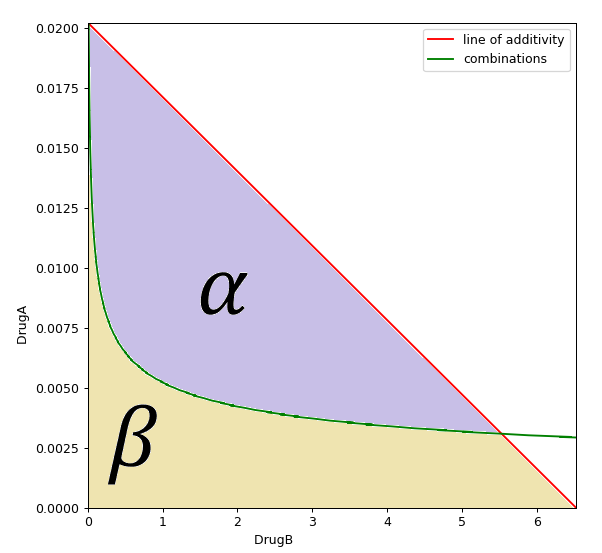
\includegraphics{../docs/iso.PNG}
\caption{}
\end{figure}

    \begin{Verbatim}[commandchars=\\\{\}]
{\color{incolor}In [{\color{incolor}25}]:} \PY{n}{C\PYZus{}a} \PY{o}{=} \PY{l+m+mi}{10}\PY{o}{*}\PY{o}{*}\PY{n}{np}\PY{o}{.}\PY{n}{array}\PY{p}{(} \PY{n}{ICs}\PY{p}{[}\PY{l+s+s1}{\PYZsq{}}\PY{l+s+s1}{x}\PY{l+s+s1}{\PYZsq{}}\PY{p}{]} \PY{p}{)}
         \PY{n}{C\PYZus{}b} \PY{o}{=} \PY{l+m+mi}{10}\PY{o}{*}\PY{o}{*}\PY{n}{np}\PY{o}{.}\PY{n}{array}\PY{p}{(} \PY{n}{ICs}\PY{p}{[}\PY{l+s+s1}{\PYZsq{}}\PY{l+s+s1}{y}\PY{l+s+s1}{\PYZsq{}}\PY{p}{]} \PY{p}{)}
         
         \PY{n}{CI} \PY{o}{=} \PY{n}{C\PYZus{}a}\PY{o}{/}\PY{l+m+mi}{10}\PY{o}{*}\PY{o}{*}\PY{n}{ICxxA} \PY{o}{+} \PY{n}{C\PYZus{}b}\PY{o}{/}\PY{l+m+mi}{10}\PY{o}{*}\PY{o}{*}\PY{n}{ICxxB}
         
         \PY{n}{idx} \PY{o}{=} \PY{n}{np}\PY{o}{.}\PY{n}{where}\PY{p}{(}\PY{n}{CI} \PY{o}{==} \PY{n+nb}{min}\PY{p}{(}\PY{n}{CI}\PY{p}{)}\PY{p}{)}
         \PY{n}{Ca\PYZus{}min} \PY{o}{=} \PY{n}{C\PYZus{}a}\PY{p}{[}\PY{n}{idx}\PY{p}{]}
         \PY{n}{Cb\PYZus{}min} \PY{o}{=} \PY{n}{C\PYZus{}b}\PY{p}{[}\PY{n}{idx}\PY{p}{]}
         
         \PY{n+nb}{print}\PY{p}{(}\PY{l+s+sa}{f}\PY{l+s+s1}{\PYZsq{}}\PY{l+s+s1}{minimum CI value [}\PY{l+s+si}{\PYZob{}}\PY{n+nb}{min}\PY{p}{(}\PY{n}{CI}\PY{p}{)}\PY{l+s+si}{:}\PY{l+s+s1}{.2f}\PY{l+s+si}{\PYZcb{}}\PY{l+s+s1}{] found at: }\PY{l+s+si}{\PYZob{}}\PY{n}{drugA}\PY{l+s+si}{\PYZcb{}}\PY{l+s+s1}{=}\PY{l+s+si}{\PYZob{}}\PY{n}{Ca\PYZus{}min}\PY{l+s+si}{\PYZcb{}}\PY{l+s+s1}{, }\PY{l+s+si}{\PYZob{}}\PY{n}{drugB}\PY{l+s+si}{\PYZcb{}}\PY{l+s+s1}{=}\PY{l+s+si}{\PYZob{}}\PY{n}{Cb\PYZus{}min}\PY{l+s+si}{\PYZcb{}}\PY{l+s+s1}{]}\PY{l+s+s1}{\PYZsq{}}\PY{p}{)}
         
         \PY{n}{idx2} \PY{o}{=} \PY{n}{np}\PY{o}{.}\PY{n}{where}\PY{p}{(}\PY{n}{CI} \PY{o}{\PYZlt{}} \PY{l+m+mi}{1}\PY{p}{)}
         \PY{n}{Ca\PYZus{}range} \PY{o}{=} \PY{n}{C\PYZus{}a}\PY{p}{[}\PY{n}{idx2}\PY{p}{]}
         \PY{n}{Cb\PYZus{}range} \PY{o}{=} \PY{n}{C\PYZus{}b}\PY{p}{[}\PY{n}{idx2}\PY{p}{]}
         
         \PY{n+nb}{print}\PY{p}{(}\PY{l+s+sa}{f}\PY{l+s+s1}{\PYZsq{}}\PY{l+s+s1}{This combination is synergistic between: }\PY{l+s+si}{\PYZob{}}\PY{n}{drugA}\PY{l+s+si}{\PYZcb{}}\PY{l+s+s1}{:[}\PY{l+s+si}{\PYZob{}}\PY{n+nb}{min}\PY{p}{(}\PY{n}{Ca\PYZus{}range}\PY{p}{)}\PY{l+s+si}{:}\PY{l+s+s1}{.3f}\PY{l+s+si}{\PYZcb{}}\PY{l+s+s1}{\PYZhy{}}\PY{l+s+si}{\PYZob{}}\PY{n+nb}{max}\PY{p}{(}\PY{n}{Ca\PYZus{}range}\PY{p}{)}\PY{l+s+si}{:}\PY{l+s+s1}{.3f}\PY{l+s+si}{\PYZcb{}}\PY{l+s+s1}{], }\PY{l+s+si}{\PYZob{}}\PY{n}{drugB}\PY{l+s+si}{\PYZcb{}}\PY{l+s+s1}{:[}\PY{l+s+si}{\PYZob{}}\PY{n+nb}{min}\PY{p}{(}\PY{n}{Cb\PYZus{}range}\PY{p}{)}\PY{l+s+si}{:}\PY{l+s+s1}{.3f}\PY{l+s+si}{\PYZcb{}}\PY{l+s+s1}{\PYZhy{}}\PY{l+s+si}{\PYZob{}}\PY{n+nb}{max}\PY{p}{(}\PY{n}{Cb\PYZus{}range}\PY{p}{)}\PY{l+s+si}{:}\PY{l+s+s1}{.3f}\PY{l+s+si}{\PYZcb{}}\PY{l+s+s1}{]}\PY{l+s+s1}{\PYZsq{}}\PY{p}{)}
         
         \PY{n}{plt}\PY{o}{.}\PY{n}{figure}\PY{p}{(}\PY{p}{)}
         \PY{n}{plt}\PY{o}{.}\PY{n}{plot}\PY{p}{(}\PY{n}{CI}\PY{p}{,} \PY{l+s+s1}{\PYZsq{}}\PY{l+s+s1}{r}\PY{l+s+s1}{\PYZsq{}}\PY{p}{,} \PY{n}{label}\PY{o}{=}\PY{l+s+s1}{\PYZsq{}}\PY{l+s+s1}{Combination Index}\PY{l+s+s1}{\PYZsq{}}\PY{p}{)}
         \PY{n}{plt}\PY{o}{.}\PY{n}{axhline}\PY{p}{(}\PY{n+nb}{min}\PY{p}{(}\PY{n}{CI}\PY{p}{)}\PY{p}{,} \PY{n}{c}\PY{o}{=}\PY{l+s+s1}{\PYZsq{}}\PY{l+s+s1}{g}\PY{l+s+s1}{\PYZsq{}}\PY{p}{,} \PY{n}{label}\PY{o}{=}\PY{l+s+s1}{\PYZsq{}}\PY{l+s+s1}{minimum CI}\PY{l+s+s1}{\PYZsq{}}\PY{p}{)}
         \PY{n}{plt}\PY{o}{.}\PY{n}{axhline}\PY{p}{(}\PY{l+m+mi}{1}\PY{p}{,} \PY{n}{c}\PY{o}{=}\PY{l+s+s1}{\PYZsq{}}\PY{l+s+s1}{b}\PY{l+s+s1}{\PYZsq{}}\PY{p}{)}
         \PY{n}{plt}\PY{o}{.}\PY{n}{xlabel}\PY{p}{(}\PY{l+s+s1}{\PYZsq{}}\PY{l+s+s1}{samples (from isobologram ICxx)}\PY{l+s+s1}{\PYZsq{}}\PY{p}{)}
         \PY{n}{plt}\PY{o}{.}\PY{n}{ylabel}\PY{p}{(}\PY{l+s+s1}{\PYZsq{}}\PY{l+s+s1}{Combination Index}\PY{l+s+s1}{\PYZsq{}}\PY{p}{)}
         
         \PY{n}{plt}\PY{o}{.}\PY{n}{legend}\PY{p}{(}\PY{p}{)}
         \PY{n}{plt}\PY{o}{.}\PY{n}{show}\PY{p}{(}\PY{p}{)}
\end{Verbatim}


    \begin{Verbatim}[commandchars=\\\{\}]
minimum CI value [0.47] found at: GSK-690693=[0.33113112], TRAMETINIB=[0.01096478]]
This combination is synergistic between: GSK-690693:[0.048-1.622], TRAMETINIB:[0.004-0.036]

    \end{Verbatim}

    
    \begin{verbatim}
<IPython.core.display.Javascript object>
    \end{verbatim}

    
    
    \begin{verbatim}
<IPython.core.display.HTML object>
    \end{verbatim}

    
    \section{CI metric}\label{ci-metric}

Rather than using min(CI), I think we should integrate the area between
the line of additivity and combination. This would be better metric of
magnitude (min CI) and also the range of concentrations at which CI is
synergistic.

Although, the \texttt{total\ area} of the plot is defined by the line of
additivity, and thus by IC50s of each single agent. We'll have to
normalize the area by this... or do we? need to think about this a
little more.

It also fits with the interpretation of \texttt{synergy} described by
plots like those below:


    % Add a bibliography block to the postdoc
    
    
    
    \end{document}
